\documentclass[a4paper]{article}
\usepackage{ctex}
\usepackage{geometry}
\usepackage{amsmath}
\usepackage{ulem}
\usepackage{graphicx}
\usepackage{siunitx}
\usepackage{enumitem}
\usepackage{multirow}
\usepackage{adjustbox}
\usepackage[hidelinks]{hyperref}
\usepackage{tabularx}
\usepackage{array}
\usepackage{float}
\newcolumntype{Y}{>{\centering\arraybackslash}X}

\geometry{left=2.5cm, right=2.5cm, top=2.5cm, bottom=2.5cm}
\zihao{-4}

\begin{document}

\noindent\textbf{班级：24级整合科学班} \hspace{1cm} \textbf{学号：2400017802} \hspace{1cm} \textbf{姓名：冯翊展} \hspace{1cm} \textbf{评分：}\\
\textbf{同组学生：无} \\
\textbf{实验名称：编写Labview质数筛程序}   \hfill \textbf{实验日期：2025年5月9日} 

\hrule
\vspace{3mm}

\begin{enumerate}[label=\chinese*.,left=0pt]
    \item 实验目的
    \\[3mm]
    学习Labview图形化编程软件，尝试使用Labview编写程序输出$10^9$之内的质数表。
  
    \item 基本原理
    \\[3mm]
    采用Eratosthenes筛法来输出所有小于 $10^9$ 的质数。其原理如下：
    \begin{enumerate}[label=\arabic*.,left=0pt]
        \item 创建一个布尔数组 $isPrime[2...n]$，初始全部标记为$true$。
        \item 从 $p=2$ 开始，若 $isPrime[p]$ 为 $true$，则将 $p$ 所有的倍数 $kp$ 标记为 $false$。
        \item 找到下一个未被标记为 $false$ 的数作为新的 $p$，重复步骤2。
        \item 当 $kp>n$ 时标记结束，将剩下所有标记为 $true$ 的位置对应的数输出。
    \end{enumerate}
    
    \item 仪器与试剂
    \\[3mm]
    电脑，Labview Community Edition 2023 Q3软件

    \item 实验结果与分析
    \\[3mm]
    使用 Labview 编写 Eratosthenes 算法程序如下：
    \begin{figure}[H]
            \centering
            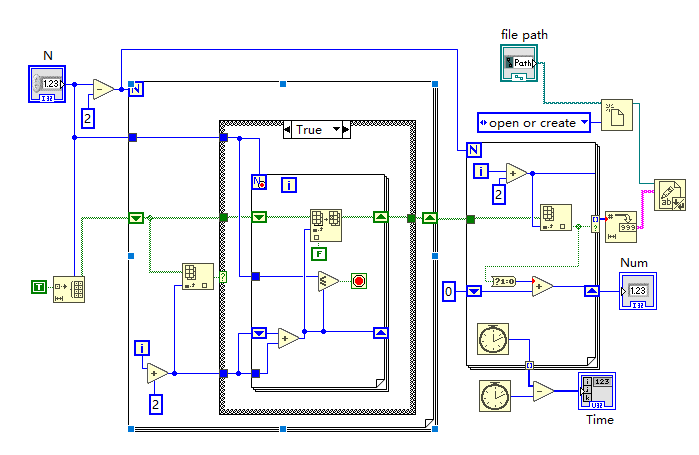
\includegraphics[width=0.9\linewidth]{Block Diagram.png}
            \caption{Block Diagram}
    \end{figure}
    设置 $n=10^9$，前面板输出如下：
    \begin{figure}[H]
        \centering
        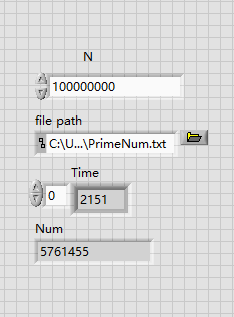
\includegraphics[width=0.4\linewidth]{Front Panel.png}
        \caption{Front Panel}
    \end{figure}
    程序运行时间为 $\qty{2151}{\ms}$，共输出 5761455 个质数，符合理论事实。

\end{enumerate}
\end{document}